\section{Software}\label{ch:software}
This chapter will talk about the software part of the project, how the design principles defined in section~\ref{ch:principles} was applied in order to solve the major obstacles before developing the application, and how the design principles helped us during the development. 

\bigskip\noindent
The first section will walk the reader through some of our keythoughts during the inital design phase of the application, and why we felt that our solutions fit within the bounderies of the design principles. 
Following this inital section we've dedicated a own section to the choice of base framework as this was one of the really major decisions during the development process and can in many cases make-or-break an application.
The second to last section will go into details about the technical aspect of the application, before we in the last section present the application as it was used during the experiments.

\subsection{Application of design principles}
In order to answer the questions proposed in the thesis while adhering to the design principles outlined we decided to utilize ideas from previous researchers within the field of educational robotics. 
One of the eariest researchers looking into how robotics could be used in schools was Seymour Papert~\cite{papert1980mindstorms}, and as a result of his research the Logo programming language was born. 
%and one of the creators of the Logo programming language were Seymour Papert (\cite{papert1980mindstorms}). 
The Logo programming language have since been implemented in numerous programs, including programs as MIT's Scratch, Turtle Art, and StarLogo TNG~\cite{logoHomepage}. Even a modified version of Scratch have created to allow for simple programming of a Arduino(S4A)~\cite{logoForArduino}. Though there exist alternatives to Logo we found that these are often uniquely coupled to a specific robot, f.ex ROBOLAB and Lego Mindstorm robot, and would most likely be close to impossible to adapt for the \chirp robot. 
%, and therefore chose to focus on implementations of the Logo language specification. 
This, coupled with the extensive research conducted using the Logo language and of the language itself~\cite{clements1990effects,clements1993research,clements1996development,clements2001logo,papert1980mindstorms}, made us decide to base our implementation on the Logo language as well. 

\bigskip\noindent
Some issues did however exist between the current implementations of Logo and our design principles. First of all is the lack of extendability and modifiability. All of them come as prepackaged solution, where modifications to the source is either not possible or extremely complex. This makes adapting the solutions to be usable in multiple settings very difficult. 
The second issues is their inherent complexity as they all implement the full Logo language specification. While this can be seen as a positive trait, we feel that the complexity of the Logo language in general is too much when using it as a mathematical tool, and would therefore like to have an option to hide some of the complexity.
The S4A implementation was created with the arduino in mind, and could have provided a good foundation for our system without the need for major modifications. The issues were however that the inherent complexity in the logo language was always exposed to the user, and that such a solution would require a laptop to create the programs for the robot.
%Who has several decades of experience with using robots as a tool in education.
%We therefore felt it natural to lean on this preexisting knowledge, and utilize the basis of Logo and its successors for our thesis. We felt this would give us a solid pedagogical fundation to start working with the application.

\bigskip\noindent
Given the issues identified with the current solutions, we decided to implement everything from the bottom up. 
As we did not need the full Logo language specification during this project, we envisioned a solution where each command was seen as a separate entity. The intent of this approach was to make the resulting solution extendable, modifiable, and open up for disabling parts of the language. 
%The full Logo language was however not needed for this project in order to mitigate this we proposed a system where parts of the programming language can be disabled to make it easier for the participants to understand and grasp. 
This way we would have the possibility of just using the commands associated with turtle graphics (e.g. \texttt{forward, backward, turn-left, turn-right}), and hide away the programming related concepts from the user.
As a natural part of basing out solution on the Logo specification we looked at the current solutions. The Scratch solution\footnote{\url{http://scratch.mit.edu/about/}} provided a block based programming interface for the specifications, something that would fit our needs perfectly in terms of usability and splitting up the language specification. 
Utilizing block-programming we were able to remove the need for writing correct syntax in order to make a program runnable, and thus increase the usability of the solution drastically. 

%In addition to basing much of the language of Logo we drew inspiration from MIT's scratch program\footnote{\url{http://scratch.mit.edu/about/}}, which is a programming tool based on predefined codeblocks. This removes the need for writing the correct syntax to make your program compile, and thus loweres the startup threshold for all participants. By utilizing a similar strategy to MIT would could allow the participants to create their program through a fully interactive graphics interface by dragging and dropping codeblocks into position. 

\bigskip\noindent
We proposed to create the system as a two component system, the \chirp robot and a programming device. 
As from the get-go we experienced trouble using the arduino integrated developer environment(AIDE), and determined that putting this system into the hands of non-technical personel would most likely deter people for using the system. 
As previous work with the robot had however shown that bluetooth was a viable option for communication between a mobile device and the robot(\cite{chrip2013ResearcherNight}), we found this to be a viable solution.
In addition a solution based on bluetooth communication would allow the system to be vastly more usable as we could remove the wired connections to a laptop, and defined our own interface in a language of our choice.
It was therefore decided that the system would use tablets(android, iPad, ect) as its programming device. This did however mean that we had to do alot of work on the application instead of reusing existing code from other projects. 

\subsubsection{Summary}
As the system was created to be used in an educational setting all the way down to lower parts of our educational system, 
we needed to make it easy to use for everyone, while still maintaining the complexity needed for children of an higher age and/or skillset. 
We wanted to create a system that could be used to teach fourth graders maths, and still be used to teach tenth graders programming at the same time. This reinforced the need for the system to be extendable, but also have an easy to use user interface. 
In order to solve this we proposed making several ways of creating the programs in the application, and making our programming modular so that subparts of the language could be disabled when not needed. To make this a feasible solution we envisioned a kernel language consisting of only actuator commands (e.g commands that directly influence the state of the robot), a extended language (which could include branching statements and variables), and a translator able to convert the extended language into the kernel language.
	
\subsection{Choice of framework}
	The first decision to be made were regarding the platform and how to achieve a crossplatform solution. 
	As solutions involving programming a computer connected to the arduino was seen as too complex we focused on frameworks aimed at mobile devices. 
	A native approach was quickly discarded as it would require multiple implementations in multiple languages (E.g. Objective-C for iOS devices, and Java for android devices, etc.). 
	Removing the native approach from our solution pool still left us with several options, including game frameworks and standardized cross platform tools.
	In a report by vision mobile in January 2013 they present a study involving six hundred developers and their preferences (\cite{developerCPT}). 
	In addition to the top five most used frameworks from vision mobile's report and some newer frameworks, we initially included game frameworks into the pool of frameworks. 
	The game frameworks were however discarded relativly fast as they rely heavily on custom built user interfaces and low level programming(openGL/webGL) for performance reasons.
	
	\bigskip\noindent
	After removing the game frameworks from our solution pool we looked throught the remaining options, PhoneGap(also known as Apache Cordova), Appcelerator, Adobe AIR, Sencha, Qt, DevExpress and Xamarin.
	
	\smalltable{Overview over potensial cross platform solutions}{table:crossplatform}{
		\begin{tabular}{lll}
			Framework & Prog. lang. & Notes\\\hline
			Apache Cordova & Javascript and HTML & \wrap{Free of charge under the apache 2 license}{0.45}\\
			Appcelerator &  Javascript & \wrap{High abstraction level. Not free to use in a commercial setting}{0.45}\\
			Adobe AIR & Flash and ActionScript & \wrap{}{0.45}\\
			Sencha & Javascript & \wrap{Commercial licensing}{0.45}\\
			Qt & C++ & \wrap{Pay to use}{0.45}\\
			DevExpress & Javascript and HTML & \wrap{Pay to use. Based on Apache Cordova technology.}{0.45}\\
			Xamarin & C\# & \wrap{Free starter pack, but have usage restrictions}{0.45}\\\hline
		\end{tabular}
	}
	
	\bigskip\noindent
	The frameworks that had commercial licenses or a "`pay to use"' business model were removed from the list of potensial frameworks, which left us with the choice between Apache Cordova, Adobe AIR and Xamarin.
	We decided to move forward with PhoneGap due to language preferences in the team. Adobe AIR, while stating that one can use javascript, does in fact require the use of Flash and ActionScript for its mobile applications, and the we had very little experience with C\#.
	Apache Cordova on the other hand is build around standard web technologies as javascript, HTML and CSS, which both members of the project have been working with before.
	
\subsection{Technical details}
With the framework decided we were able to start creating our system. 
Throughout the process of creating the application we focused on refactoring options, configurations and settings in each component into their own components. These options/settings would at a later stage be gathered together and some were exposed through the user interface in order to make it possible to change the behaviour of the application at runtime. The process of always putting all the configuration and options in the same place made it possible for the system to be extremely extendable and modifiable. 

\bigskip\noindent
The main part of the application were developed using javascript, HTML and CSS, as these are the primary technologies used when creating application with the Apache Cordova framework. We will therefore keep the focus on these technologies, even though some minor adjustments where done in the native android controller to enable a higher debugging level than the bluetooth plugin had originaly.

\bigskip\noindent
Figure~\ref{fig:class} shows a simple "`class diagram"' of the application as it was when the project was coming to an end. Note that the term class diagram is not completely accurate as javascript is not a object oriented programming language in the same sense as Java, but utilizes prototypical inheritance to reuse common code components. The code for this application however isn't powered by a complicated class hierarchy and thus using the "`class diagram"' is sufficient to show how different components interact.

\image{images/class.png}{\linewidth}{"`Class diagram"' of the javascript application.}{fig:class}

\bigskip\noindent
The class diagram in figure~\ref{fig:class} shows a total of eighteen different javascript files, most of whom contain a single javascript "`class"', though some do contain several classes, but these classes are at an abstraction level below what should be exposed by the parent class. 

\bigskip\noindent
The main responsibilities of each class is shown in table~\ref{table:technical}.
\begin{center}
	\begin{longtable}{ll}
		\hline
		\textbf{Class name} & \wrap{\textbf{Descriptions}}{0.6}\\
		\hline
		\endfirsthead
		
		\multicolumn{2}{c}{{
			\bfseries \tablename\ \thetable{} -- continued from previous page
		}}\\\endhead
		
		\\
		\multicolumn{2}{c}{
			\textbf{Continued on next page}
		}\\\hline\endfoot
		\endlastfoot
		
		\textbf{main.js} & \wrap{Provides the entrypoint for the application. This file does not contain any classes, but have the responsibility of starting the application up, initializing all the other classes and handling the majority of events delegation.}{0.6}\\
		\textbf{Program.js} & \wrap{Provides the Program class, which is responsibel for the extraction and validation of the program from either the graphical interface or the textual interface.}{0.6}\\
		\textbf{RunnableProgram.js} & \wrap{Is a wrapper around the Program model responsible for preparsing of the program in the cases where pure javascript have been written.}{0.6}\\
		\textbf{Options.js} & \wrap{A centralized locations for all application settings. Provides persistent storage of settings, and a simple user interface creator for generating the options menu.}{0.6}\\
		\textbf{Keyboard.js} & \wrap{A simple class responsible for creating and handling a on-screen-keyboard.}{0.6}\\
		\textbf{Codeblock.js} & \wrap{Another model class which stores the information of a single command. Marshalling and unmarshalling from and to the graphical and textual interface are handled by this model, but usually called at the \textit{Program} level.}{0.6}\\
		\textbf{CodeblockManager.js} & \wrap{Responsible for inserting available codeblocks into the header of the application, and helping with the marshalling of textual blocks.}{0.6}\\
		\textbf{CodeblockDefinitions.js} & \wrap{Provides the definition of all available codeblocks in the system, and how the different codeblocks should be translated into javascript. }{0.6}\\
		\textbf{Device.js} & \wrap{An abstraction layer for removing any device dependencies and allowing the application to be tested on a computer by mocking different device dependent components.}{0.6}\\
		\textbf{jsEngine.js} & \wrap{A generator class responsible for converting the Program or pure javascript into actual commands which can be sent to the robot.}{0.6}\\
		\textbf{SimulatorFactory.js} & \wrap{The class responsible for keeping track of which of the four simulator types to use. This class listens to changes in bluetooth connectivity in order to allways provide the correct simulator.}{0.6}\\
		\textbf{*Simulator.js} & \wrap{Refers to all the differet simulators. These classes takes a RunnableProgram as the argument, and spins up the correct simulator. In cases where a robot is connected they also have the responsibility of sending the commands and keeping in sync with the robot.}{0.6}\\
		\textbf{*Bluetooth.js} & \wrap{Refers to both bluetooth classes. Based on a debugging flag in the application one of these classes will be started. MockBluetooth will keep the same to the same interface as Bluetooth, but will use stubbing methods in order to provide a testing surface for the bluetooth functionality.}{0.6}\\
		\textbf{ConnectionUI.js} & \wrap{The bluetooth connection user interface is dynamically injected if a bluetooth enabled device is detected by the application. The UI is maintained by this class.}{0.6}\\
		\caption{Class descriptions}\label{table:technical}
	\end{longtable}
\end{center}

\bigskip\noindent
As can be seen from the class diagram in figure~\ref{fig:class}, there is a lot of connected components within the application. 
This architecture was chosen in order to make each component's  responsibility as small and concrete as possible, which prevents alot of ripples if one component should change and helps identify the location of bug. 

\bigskip\noindent
Most of the classes/files in the application are straight forward javascript "`classes"' with a minimal responsibility, which make them straightforward to understand and debug. The exception to this may be the application backbone responsible for translating our internal program representation into a program which can run on the robot and the simulator. Because of this, and all the other interactions between the components, we've included a short sequence diagram and explaination of how the application works when a user tries to start his or her program. 

\bigskip\noindent
The diagram starts off with the user initiating the \texttt{Run} sequence, telling the application to take the currect program and run it. 
The \texttt{Program} class retrieves the program either from the graphical input or from the textual input dependent on which were active at the time when the user started the sequence. The program is at this program replaces by an instance of \texttt{RunnableProgram}, see listing~\ref{lst:loop}.
When the program have been retrieved and converted the event handler requests a simulator from the \texttt{simulatorFactory}, which in turn determines the currect \texttt{simulator} given the current state of the application(e.g. if a bluetooth connection is actice). 
With the simulator and runnable program prepared the event handler sends the program to the simulator and lets the simulator take it from there.
The simulator will at this point request a program generator from the runnable instance.
The program generator will if necessary convert the program into javascript(listing~\ref{lst:internal}), sandbox the newly created javascript code and run it to generate the output commands needed for the simulator. The commands(listing~\ref{lst:commands}) are at this point presented in a similar fashion to what you would expect from an java iterator (\texttt{hasNext} and \texttt{next} commands). With the support for native generator coming to javascript with the new ECMAscript 6 standard this is self created generator is most likely to be exchanged in favor of a native approach (\cite{mozillaES6}).
If a bluetooth connection is present at this point and the simulator support bluetooth synchronization it will try to send the commands to the robot. 

\bigskip\noindent
In order to contain most of the complexity within the application and not on the arduino we translate the commands into simple \texttt{move} and \texttt{turn} commands for the bluetooth module. A move command would be prefixed with the letter \texttt{m}, followed by a either a \texttt{+} or \texttt{-} indication the direction (positive is forward), and four hex-digits indication the length. I similar structure was used for turn commands with the prefix \texttt{t} instead of \texttt{m} (positive is a right turn).

\image{images/sequence.png}{0.9\linewidth}{Sequence diagram of initialization of a user program}{fig:sequence}

\bigskip\noindent
The code snipplets (listings~\ref{lst:loop} and~\ref{lst:internal}) were choosen here as an example due to the fact that most of the language currently implemented is showcased in the example. This is however the extended mode of the language, whereas the experiment was conducted without loops, procedures and variables enabled in the language. Another reason for using this rather overly complex example is to give a thorough presentation of the internal representation (e.g. how the halting program is solved by limiting the number of total commands).

\bigskip\noindent
It should be noted that the inital solution to translate the user program into robot commands were done by our own simple translater. This did however become infeasble to maintain as the application language evolved and started to touch on more advanced programming structures as loops and procedures.  

\begin{minipage}{\linewidth}
	\begin{lstlisting}[frame=single,numbers=left,caption={Example code for creating a square using variables (Extended language), procedures and loop.},language=MyBasic,label=lst:loop]
SET NUM 4
SET LENGTH 100
SET ANGLE 90
PROC SEGMENT
    FWD LENGTH
    TL ANGLE
END 
REP NUM
    CALL SEGMENT
END 
	\end{lstlisting}
%\end{minipage}
%\begin{minipage}{\linewidth}
	\begin{lstlisting}[frame=single,numbers=left,caption={Commands sent to simulator(Kernel language)},language=MyBasic,label=lst:commands]
FWD 100
TL 90
FWD 100
TL 90
FWD 100
TL 90
FWD 100
TL 90
	\end{lstlisting}
\end{minipage}
\begin{minipage}{\linewidth}
	\begin{lstlisting}[frame=single,numbers=left,caption={The internal representation of the previous program.},language=Javascript,label=lst:internal]
var icount = 0; 

SET("NUM", 4);var NUM = 4; 
SET("LENGTH", 100);var LENGTH = 100; 
SET("ANGLE", 90);var ANGLE = 90; 

function SEGMENT() { 
	icount++; 
	if (icount > 30000){return;} 
	FWD(LENGTH); 

	icount++; 
	if (icount > 30000){return;} 
	TL(ANGLE); 
	END();
} 

REP(NUM);
for (var generated_55033 = 0; generated_55033 < NUM;generated_55033++) { 
	CALL("SEGMENT");
	SEGMENT(); 
	END();
}
	\end{lstlisting}
\end{minipage}

\subsection{Resulting application}
The final version of the application\footnote{\texttt{v1.1} in \url{https://bitbucket.org/nutgaard/turtle/commits/all}} created a easy to use, extendable, crossplatform, and modifiable environment for creating program to the robot regardless of previous experience with programming and robotics. As the application also works as an web application (with the exception of bluetooth) we've deployed the application to web as well\footnote{\url{http://folk.ntnu.no/nicklau/turtle/}}. The web application is initialized with a mock instance of the bluetooth module, hence the application behaves exactly as if on a mobile device (appendix~\ref{appendix:appIntro} gives an introduction to the usage of the application). 

\bigskip\noindent
For the non-technical users the application provides a graphical user interface where the user simply can drag the commands around and create the program without ever needing to know anything about programming or internal syntaxes. For more experienced users the application provides a textural interface, where the user can either write the code using the applications own language(listing~\ref{lst:loop}), or pure javascript code. 

\bigskip\noindent
In additions to being able to change the complexity of how the program are created the application provides options for disabling parts of the language. In its simplest form the application provides only four commands, forward, backward, turn left, and turn right (figure~\ref{fig:appAugmented}). 

\begin{figure}
	\centering
	\subfloat[Complete application\label{fig:appAugmented}]{
		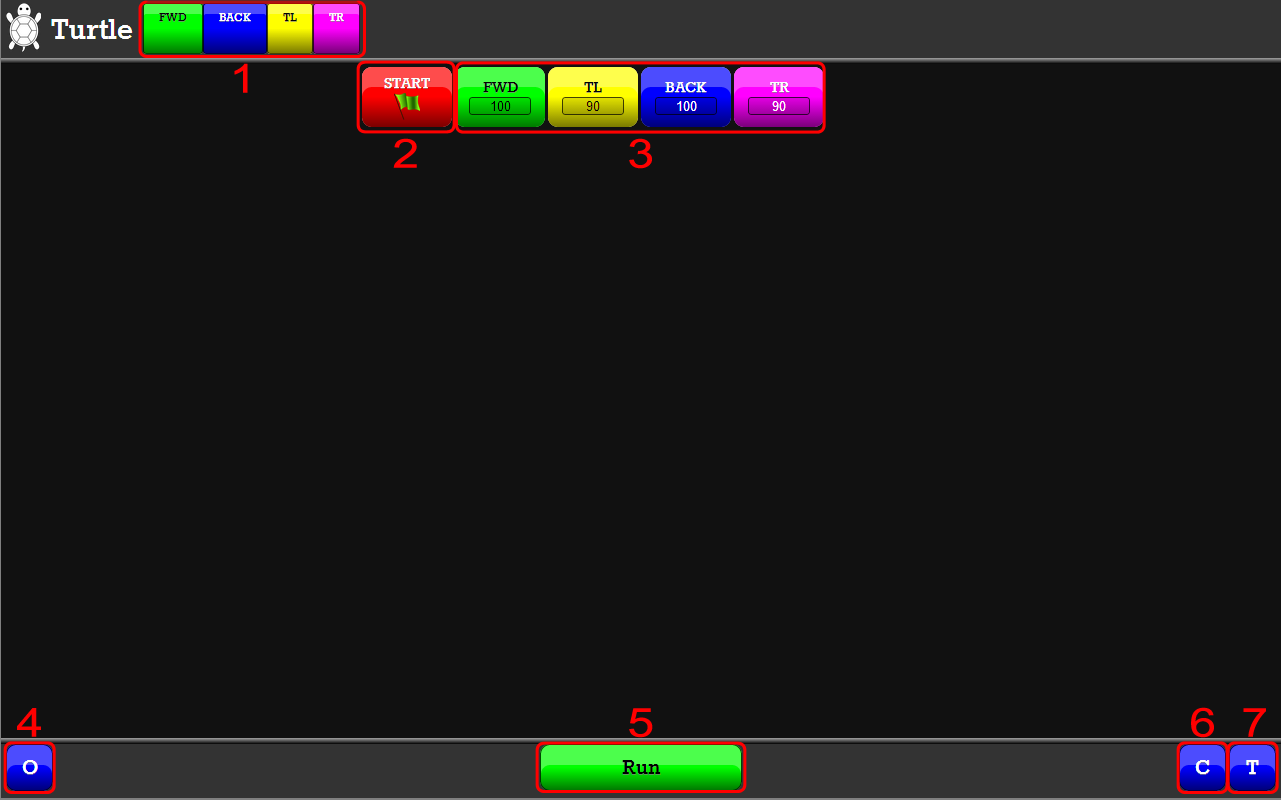
\includegraphics[width=0.45\linewidth]{images/app/SimpleMainAugmented.png}
	}
	\subfloat[Simulator view\label{fig:appSimulator}]{
		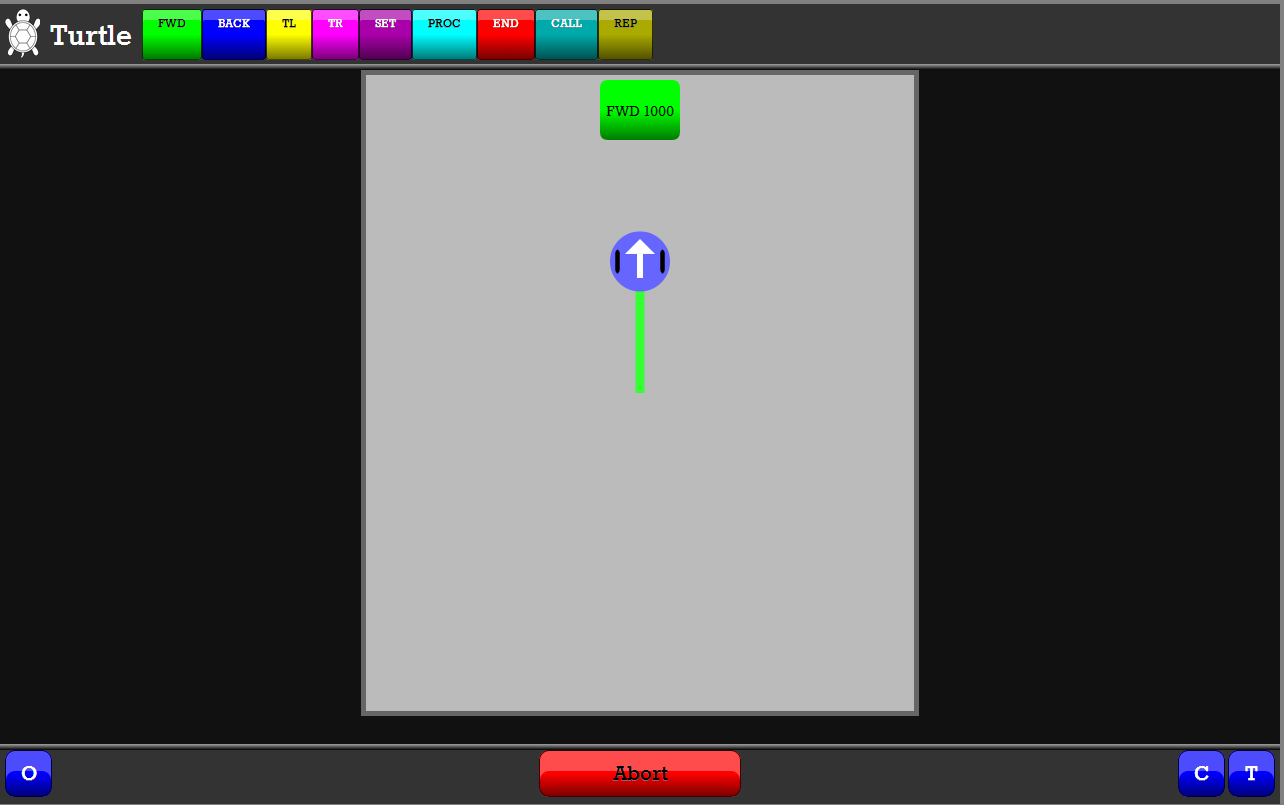
\includegraphics[width=0.45\linewidth]{images/app/Simulator.png}
	}
\end{figure}

\bigskip\noindent
For a complete introduction to the usage of the application please refer to appendix~\ref{appendix:appIntro}, where the whole application, including the different simulators, options, and programming styles, is presented.